%%%%%%%%%%%%%%%%%%%%%%%%%%%%%%%%%%%%%%%%%
% Friggeri Resume/CV
% XeLaTeX Template
% Version 1.0 (5/5/13)
%
% This template has been downloaded from:
% http://www.LaTeXTemplates.com
%
% Original author:
% Adrien Friggeri (adrien@friggeri.net)
% https://github.com/afriggeri/CV
%
% License:
% CC BY-NC-SA 3.0 (http://creativecommons.org/licenses/by-nc-sa/3.0/)
%
% Important notes !!! : 
% Use texshop for better editor and this template needs to be compiled with XeLaTeX and the bibliography, if used,
% needs to be compiled with bibtex with biber backend.
%
%%%%%%%%%%%%%%%%%%%%%%%%%%%%%%%%%%%%%%%%%

\documentclass[style=verbose,maxnames=99,sorting=ydnt,style=verbose,maxnames=99,sorting=ydnt,backend=biber]{friggeri-cv} % Add 'print' as an option into the square bracket to remove colors from this template for printing



\addbibresource{cv-dhoto.bib} % Specify the bibliography file to include publications

%\usepackage[style=verbose,maxnames=99,sorting=ydnt,backend=biber]{biblatex}
\usepackage{fancyhdr}

\usepackage{lastpage}
 
\pagestyle{fancy}
\fancyhf{}
 
\rfoot{CV-Dhoto - Page \thepage \hspace{1pt} of \pageref{LastPage}}

\usepackage{wrapfig}
\usepackage[super]{nth}

\usepackage{lipsum}
%------------
\usepackage{enumitem}
\renewenvironment{entrylist}{%
  \begin{itemize}[leftmargin=1in]%[leftmargin=*,align=left,itemindent=-\dimexpr\labelwidth+\labelindent+\labelsep\relax]
}{%
  \end{itemize}
}
\renewcommand{\bfseries}{\headingfont\color{headercolor}}
\renewcommand{\entry}[4]{%
  \item[#1]
    \textbf{#2}%
    \hfill%
    {\footnotesize\addfontfeature{Color=lightgray} #3}\\%
    #4\vspace{\parsep}%
  }
%-------


\begin{document}

\header{Sritrusta}{ Sukaridhoto}{Assistant Professor, Technology Enthusiast and Guitarist} % Your name and current job title/field

%----------------------------------------------------------------------------------------
%	SIDEBAR SECTION
%----------------------------------------------------------------------------------------

\begin{aside} % In the aside, each new line forces a line break
\section{contact}
\textbf{Politeknik Elektronika Negeri Surabaya}
Gedung Pascasarjana \nth{9} Floor, Room: PS09.03
Jl. Raya ITS Surabaya
~
Office:+62 (31) 5947280 ext:7902
Mobile:+62 823 6666 6379
Email: \href{mailto:dhoto@pens.ac.id}{dhoto@pens.ac.id}
~
\href{http://dhoto.lecturer.pens.ac.id/}{Dhoto's Homepage}
\href{https://scholar.google.co.id/citations?user=M6sGfNQAAAAJ&hl=en&oi=ao}{Google Scholar}
\href{https://www.scopus.com/authid/detail.uri?authorId=35100882700}{Scopus-ID}
\href{http://github.com/iseng4h}{git://iseng4h}
\href{http://facebook.com/iseng4h}{fb://iseng4h}
\section{languages}
Indonesian (native)
English \& Japanese 
\section{research interests}
{\color{red} $\varheartsuit$} Computer Networks,
Human-centric, Multimedia \& Internet of Things
\end{aside}

%----------------------------------------------------------------------------------------
%	MAIN SECTION
%----------------------------------------------------------------------------------------

\section{biography}

\begin{wrapfigure}[10]{l}{1.5in}
	\vspace{-10pt}
	\begin{center}
    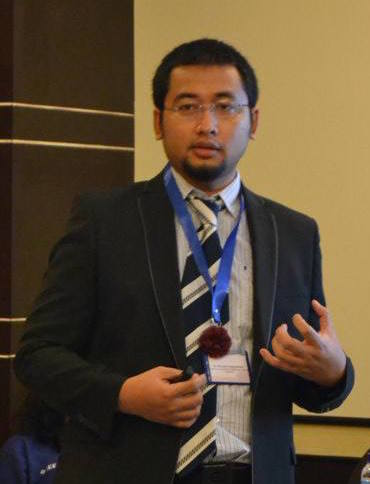
\includegraphics[width=0.2\textwidth]{dhoto-jas.jpg}
    \end{center}
    
\end{wrapfigure}
Received the B.E. degree in electrical engineering, computer science program from Sepuluh Nopember Institute of Technology, Indonesia, in 2002 and the Ph.D. degree in Communication Networks Engineering from Okayama University, Japan, in 2013. He joined at Politeknik Elektronika Negeri Surabaya, Indonesia, as a lecturer in 2002. He stayed at Tohoku University, Japan, in 2004, as a visiting researcher. From 2017, He becomes Head of Human Centric Multimedia Lab, received several research grants, and also has several collaborations with government and industries. He is a technology enthusiast, his research interests include computer networks, human-centric, immersive multimedia technology, and Industrial Internet of Things. He has received several academic awards, best paper awards, and IEEE Young Researcher Award in 2009. He is a member of IEEE.



\section{education}

\begin{entrylist}
%------------------------------------------------

\entry
{2009--2013}
{Doctor {\normalfont of Philosophy}}
{Okayama University, Japan}
{\emph{Engineering} \\ 
Dissertation: "A Study of Performance Improvement Methods for Real-Time Applications in Wireless Mesh Networks" \\
Supervised by Prof. Nobuo Funabiki, Prof. M. Hata and Prof. Toru Nakanishi}

%------------------------------------------------
\entry
{1997--2002}
{Bachelor {\normalfont of Engineering}}
{Institut Teknologi Sepuluh Nopember, Indonesia}
{Electrical Engineering - Computer Science\\
Thesis: “Implementation of IPv6 in Institute Technology Sepuluh November of Surabaya” 
\\Supervised by Dr. Surya Sumpeno and Dr. Supeno Mardi
}

%------------------------------------------------
\end{entrylist}

%----------------------------------------------------------------------------------------
%	WORK EXPERIENCE SECTION
%----------------------------------------------------------------------------------------

\section{work experience}

\begin{entrylist}
%------------------------------------------------
\entry
{2002-Now}
{Politeknik Elektronika Negeri Surabaya}
{Surabaya, Indonesia}
{\emph{Assistant Professor \& Head of Lab} 
\begin{itemize}
\item Graduate School of Information Technology, 
\begin{itemize}
\item Teaching : Advanced Computer Networks and Internet of Things
\item Supervision of Master students
\end{itemize}
\item Department of Multimedia Creative Technology, 
\begin{itemize}
\item Teaching : Data Communication and Computer Networks
\item Supervision of Undergraduate students
\end{itemize}
\item Head of Human Centric Multimedia Lab
\end{itemize}
}

%------------------------------------------------
\entry
{2019-now}
{PT. Daitan Citra Global (TANTRA)}
{Bekasi, Indonesia}
{\emph{Research n Development}, we develop solution and integration in the industrial, manufacture, and IT.}

%Masih berlangsung
\entry
{2019-now}
{Agile and Young, PT. Solusi Integra Indonesia}
{BSD, Indonesia}
{\emph{Chief technology officer}, startup that working on solution and integration in the field of oil and gas, manufacture, and IT.}

\entry
{2019-2021}
{Dinas Kependudukan dan Catatan Sipil}
{Surabaya, Indonesia}
{\emph{IT Consultant}}

\entry
{2017, 2018}
{Bank Jatim}
{Surabaya, Indonesia}
{\emph{IT Consultant}}

\entry
{2018}
{Artha Patria - Softwate Development}
{Surabaya, Indonesia}
{\emph{CTO}, we develop software for human resource management. Our clients: PT. Quantum, Inasgoc2018, BPKH, etc}

%------------------------------------------------
%Sudah selesai

\entry
{2015-2018}
{UGT Sidogiri - USAT}
{Pasuruan, Indonesia}
{\emph{Internet Service Provider Consultant}}


\entry
{2017, 2018}
{PT. Eyro Digital Technology}
{Surabaya, Indonesia}
{\emph{IoT, Big Data architecture Consultant}}

\entry
{2016}
{Dinas Komunikasi dan Informatika}
{Surabaya, Indonesia}
{\emph{Network Security Consultant}}

\entry
{2014, 2019}
{PT PAL SURABAYA - Kementrian Pertahanan dan Keamanan RI}
{Okpo, Korea}
{\emph{Research and Development of National Submarine} Transfer of Technology, national research collaboration and Submarine design for weapon system, communication, and computer system}
%------------------------------------------------
\entry
{2004-2009}
{Politeknik Elektronika Negeri Surabaya}
{Surabaya, Indonesia}
{\emph{CISCO Network Academy Instructor}}


\entry
{1999-2002}
{Institut Teknologi Sepuluh Nopember}
{Surabaya, Indonesia}
{\emph{Network Administrator} of its.ac.id, manage all network devices such as switches, routers and servers.}

\entry
{1999-2002}
{Judistira Webhosting}
{Surabaya, Indonesia}
{\emph{Network Administrator} of web hosting provider, manage all servers and web developer}


\end{entrylist}


\section{research experience}

\begin{entrylist}

%----------------------------------------------
\entry
{2017-Now}
{Human Centric Multimedia}
{Surabaya, Indonesia} 
{\emph{Head of Lab} \\
Research about Multimedia and Internet of Things
\begin{itemize}
\item Augmented and Virtual Reality
\item Human-Centric, Interaction with Computer Vision and Speech Recognition-Understanding
\item Internet of Things and BigData
\item Application of Machine Learning and Artificial Intelligence
\end{itemize}
}

%----------------------------------------------
\entry
{2013-2017}
{EEPIS Robotics Research Center (ER2C)}
{Surabaya, Indonesia} 
{\emph{Senior Researcher} \\
Research about Cyber-Physical Systems
\begin{itemize}
\item MicroKernel OS for Embedded System
\item Human Robot Interaction with Computer Vision and Speech Recognition-Understanding
\item Internet of Things and BigData
\end{itemize}
}

%----------------------------------------------
\entry
{2008-2013}
{Distributed System Lab, Okayama University}
{Okayama, Japan} 
{\emph{Research Assistant} under supervised by Prof. Nobuo Funabiki\\
Research about Communication Networks
\begin{itemize}
\item Wireless Mesh Networks
\item Real-time wireless communication
\item Mac protocol
\end{itemize}
}

%----------------------------------------------
\entry
{2004-2008}
{Computer Network Units of EEPIS}
{Surabaya, Indonesia} 
{Research on 
\begin{itemize}
\item Computer Networks
\item Computer Vision and Speech Recognition
\item Integrity Systems
\end{itemize}
}

%------------------------------------------------
\entry
{2003-2004}
{Tohoku University}
{Sendai, Japan}
{\emph{Visiting Reseacher} under supervised by Prof. Takafumi Aoki\\
Research on 
\begin{itemize}
\item Biometric Fingerprint Matching
\item Parallel Computing
\item Embedded System
\end{itemize}
}

\end{entrylist}

%--------------
% SOCIETY
%--------------

\section{society}

\begin{entrylist}

\entry
{2020-now}
{International Journal of Web Information Systems}
{Emerald Group Publishing}
{Reviewer}

\entry
{2020-now}
{Indonesia Journal of Artificial Intelligence}
{Institute of Advanced Engineering and Science (IAES)}
{Reviewer}

\entry
{2020-now}
{Indonesia Journal of Electrical Engineering and Computer Engineering}
{Institute of Advanced Engineering and Science (IAES)}
{Reviewer}


\entry
{2020-now}
{Indonesia Journal of Electrical Engineering and Computer Science}
{Institute of Advanced Engineering and Science (IAES)}
{Reviewer}

\entry
{2019-now}
{TELKOMNIKA}
{Universitas Ahmad Dahlan (UAD)}
{Reviewer}

\entry
{2020-now}
{Indonesia Journal of Electrical Engineering and Computer Science}
{Institute of Advanced Engineering and Science (IAES)}
{Reviewer}

\entry
{2019-now}
{Reviewer Penelitian Nasional}
{RISTEKBRIN}
{Reviewer}

\entry
{2019-now}
{Asosiasi Pengusaha TIK Nasional}
{Indonesia}
{Member}

\entry
{2016, 2019}
{IEEE - International Electronics Symposium}
{Bali, Indonesia}
{General Chair}

\entry
{2018}
{IC2IE - International Conference of Computer and Informatics Engineering}
{Bogor, Indonesia}
{Keynote Speaker}

\entry
{2018}
{SEHATI - Seminar Nasional Humaniora dan Aplikasi Teknologi Informasi}
{Madura, Indonesia}
{Keynote Speaker}




\entry
{2015-now}
{IAENG Member}
{}
{Membership number: 159948}

\entry
{2009-now}
{IEEE Member}
{}
{Membership number: 90775049}




\end{entrylist}


%----------------------------------------------------------------------------------------
%	AWARDS SECTION
%----------------------------------------------------------------------------------------
%\pagebreak
\section{award and certification}

\begin{entrylist}
%------------------------------------------------
\entry
{2020}
{Exin Agile Scrum Master}
{EXIN}
{\href{https://app.exeed.pro/holder/badge/72572}{Credential Link}}

\entry
{2020}
{Exin Agile Scrum Foundation}
{EXIN}
{\href{https://app.exeed.pro/holder/badge/70331}{Credential Link}}

\entry
{2020}
{AgilePM Foundation}
{APMG International}
{\href{https://www.credly.com/badges/97b301f8-af16-45e1-a45c-ead6c1cc4d9b/linked_in_profile}{Credential Link}}

\entry
{2020}
{ISO27001 Lead Auditor - Information Security Certification}
{Intertek}
{ID: 211206}

\entry
{2020}
{CertNexus Certified Internet of Things Practioner (CIOTP)}
{CertNexus}
{\href{https://www.credential.net/685c1367-a0d4-40ba-894f-08601040276f}{Credential link}}

\entry
{2020}
{Pro Tools Certified User}
{AVID}
{\href{https://training.digidesign.com/listings/listing_admin/user_cert4.cfm?id=8236457&courseid=428}{Credential link}}

\entry
{2019}
{Best Paper Award}
{IES2019, Indonesia}
{\emph{Designing of a Smart Collar for Dairy Cow Behavior Monitoring with Application Monitoring in Microservices and Internet of Things-Based Systems}, Yogi Putra Pratama, Dwi Kurnia Basuki, Sritrusta Sukaridhoto, Alviansyah Arman Yusuf, Heri Yulianus, Faruq Faruq, Fariz Bramasta Putra;  (2019 International Electronics Symposium (IES)), Indonesia}


%------------------------------------------------
\entry
{2018}
{Best Paper Award}
{TELKOMNIKA, Indonesia}
{\emph{Implementation Integration of VaaMSN with SEMAR for Air Monitoring Solution}, Yohanes Yohanie Fridelin Panduman, Adnan Rachmat Anom Besari, Sritrusta Sukaridhoto, Rizqi Putri Nourma Budiarti, Rahardhita Widyatra Sudibyo, Funabiki Nobuo; TELKOMNIKA (Telecommunication Computing Electronics and Control), Indonesia}


%------------
\entry
{2013-2016}
{Dosen Joss}
{Politeknik Elektronika Negeri Surabaya}
{Annual award for the best lecturer in department.}
%------------------------------------------------
\entry
{2014}
{Best Paper Award}
{The 16th International Electronics Symposium, Indonesia}
{\emph{Application Programming Interface Design of Microkernel Based Robotics Operating System}, Adhe Widianjaya, Dadet Pramadihanto, Sritrusta Sukaridhoto; The 16th International Electronics Symposium, Indonesia}


%------------
\entry
{2009}
{IEEE’s Young Researcher Award}
{ISCE2009, Japan}
{}
%------------------------------------------------
\entry
{2009}
{Monbusho Scholarship for Doctoral Program}
{Okayama University, Japan}
{}
%------------------------------------------------
\entry
{2008}
{CCNA Certified}
{CISCO}
{CISCO ID : CSCO11381768}
\entry
{2007}
{Best Paper Award}
{Seminar Nasional Open-Source Software ke-2, Indonesia}
{\emph{“Sistem Pendeteksi Gambar Porno”}, Dadet Pramadihanto, Sritrusta Sukaridhoto, Muhammad Fatoni A, Rudy Cahyadi H; Prosiding Seminar Nasional Open Source Software ke-2 2007 
}
%------------------------------------------------
\end{entrylist}

%---------------------
%Research Grant
%--------------------

\section{research grants}

\begin{entrylist}
\entry
{2020}
{Implementasi Vehicle as a Mobile Sensor Network terintegrasi dengan Smart Environment Monitoring and Analytics in Real-time (SEMAR) system sebagai Pemantau Permukaan Jalan dan Lingkungan untuk mendukung Smart City
}
{DIKTI}
{Penelitian Terapan Unggulan Perguruan Tinggi (Lead) - year: 3 of 3 - Rp. 143.310.000,-}

\entry
{2020}
{Implementasi Teknologi Portable Ubiquitous Health (U-Health) Dengan Layanan Cloud Untuk Mendukung Smart Health Buatan Indonesia
}
{DIKTI}
{Penelitian Terapan Unggulan Perguruan Tinggi - year: 3 of 3 - Rp. 132.860.000,-}
\entry
{2019}
{Implementasi Vehicle as a Mobile Sensor Network terintegrasi dengan Smart Environment Monitoring and Analytics in Real-time (SEMAR) system sebagai Pemantau Permukaan Jalan dan Lingkungan untuk mendukung Smart City
}
{DIKTI}
{Penelitian Terapan Unggulan Perguruan Tinggi (Lead) - year: 2 of 3 - Rp. 143.310.000,-}

\entry
{2019}
{Implementasi Teknologi Portable Ubiquitous Health (U-Health) Dengan Layanan Cloud Untuk Mendukung Smart Health Buatan Indonesia
}
{DIKTI}
{Penelitian Terapan Unggulan Perguruan Tinggi - year: 2 of 3 - Rp. 132.860.000,-}

\entry
{2019}
{INTELIGENT SYSTEM DEVELOPMENT FOR AUTOMATIC CLASSIFICATION OF FRUIT DEFECT}
{DIKTI}
{Penelitian Kompetitif Nasional ( PPS-PTM ) - year: 1 of 1 - Rp. 49.600.000,-}


\entry
{2018}
{Implementasi Vehicle as a Mobile Sensor Network terintegrasi dengan Smart Environment Monitoring and Analytics in Real-time (SEMAR) system sebagai Pemantau Permukaan Jalan dan Lingkungan untuk mendukung Smart City
}
{DIKTI}
{Penelitian Terapan Unggulan Perguruan Tinggi (Lead) - year: 1 of 3 - Rp. 120.000.000,-}

\entry
{2018}
{Implementasi Teknologi Portable Ubiquitous Health (U-Health) Dengan Layanan Cloud Untuk Mendukung Smart Health Buatan Indonesia
}
{DIKTI}
{Penelitian Terapan Unggulan Perguruan Tinggi (Member) - year: 1 of 3 - Rp. 120.000.000,-}

\entry
{2018}
{Revitalisasi Sistem Jejaring Radio HF Untuk Mendukung Implementasi Jejaring Radio Pemerintah – GRN
}
{DIKTI}
{Penelitian Terapan Unggulan Perguruan Tinggi (Member) - year: 1 of 3 - Rp. 130.000.000,-}

\entry
{2018}
{Pusat Pendidikan dan Pelatihan Embedded System Bersertifikasi Sebagai Upaya Penyiapan Sumber Daya Manusia Menjelang Masyarakat Ekonomi ASEAN}
{DIKTI}
{Ipteks Bagi Inovasi Kreativitas Kampus (Member) - year: 3 of 3 - Rp. 150.000.000,- + Rp 50.000.000,-}

\entry
{2018}
{Industrial Edge Computing}
{CISCO System Indonesia}
{inKind}

\entry
{2018}
{Industrial Internet of Things}
{Ichii Industries Indonesia}
{inKind}

\entry
{2018}
{IoT - Smartglass for Industrial Factory Assistant}
{TMMIN}
{inKind}

\entry
{2017}
{DESIGN AND DEVELOPMENT OF UNMANNED UNDERWATER VEHICLES FOR ENVIRONMENTAL MONITORING AND DATA ACQUISITION COMPATIBLE WITH 5D WORLD MAP SYSTEM IN INTERNET OF UNDERWATER THINGS}
{DIKTI}
{Penelitian Kerjasama Luar Negeri dan Publikasi International - year: 3 of 3 - Rp. 151.000.000,-}

\entry
{2017}
{Pusat Pendidikan dan Pelatihan Embedded System Bersertifikasi Sebagai Upaya Penyiapan Sumber Daya Manusia Menjelang Masyarakat Ekonomi ASEAN}
{DIKTI}
{Ipteks Bagi Inovasi Kreativitas Kampus - year: 2 of 3 - Rp. 189.000.000,- + Rp 50.000.000,-}

\entry
{2017}
{Industrial Internet of Things}
{Ichii Industries Indonesia}
{inKind}

\entry
{2017}
{CSR for Robotics and IoT}
{TMMIN}
{inKind}

\entry
{2016}
{DESIGN AND DEVELOPMENT OF UNMANNED UNDERWATER VEHICLES FOR ENVIRONMENTAL MONITORING AND DATA ACQUISITION COMPATIBLE WITH 5D WORLD MAP SYSTEM IN INTERNET OF UNDERWATER THINGS}
{DIKTI}
{Penelitian Kerjasama Luar Negeri dan Publikasi International - year: 2 of 3 - Rp. 160.000.000,-}

\entry
{2016}
{Pusat Pendidikan dan Pelatihan Embedded System Bersertifikasi Sebagai Upaya Penyiapan Sumber Daya Manusia Menjelang Masyarakat Ekonomi ASEAN}
{DIKTI}
{Ipteks Bagi Inovasi Kreativitas Kampus - year: 1 of 3 - Rp. 189.000.000,- + Rp 50.000.000,-}


\entry
{2015}
{DESIGN AND DEVELOPMENT OF UNMANNED UNDERWATER VEHICLES FOR ENVIRONMENTAL MONITORING AND DATA ACQUISITION COMPATIBLE WITH 5D WORLD MAP SYSTEM IN INTERNET OF UNDERWATER THINGS}
{DIKTI}
{Penelitian Kerjasama Luar Negeri dan Publikasi International - year: 1 of 3 - Rp. 157.500.000,-}

\entry
{2015}
{Virtual Reality Lab sebagai penunjang Perkuliahan Terbuka Jarak Jauh (PTJJ)}
{Seamolec}
{Penelitian Hibah PTJJ Seamolec - Rp 10.000.000,-}

\entry
{2014}
{PENGEMBANGAN ARSITEKTUR KOMPUTASI DAN SISTEM OPERASI ROBOTIKA UNTUK PENINGKATAN DAYA SAING APLIKASI ROBOTIKA NASIONAL}
{DIKTI}
{Penelitian Unggulan Perguruan Tinggi - year: 2 of 5 - Rp 200.000.000,-}

\entry
{2005}
{Rancang Bangun Prototype Mesin Verifikasi Sidik Jari Compact and Mobile dengan Algoritma Phase-Only Correlation  Berbasis Embedded System}
{DIKTI}
{Penelitian Hibah Bersaing - Rp 40.000.000,-}

\entry
{2005}
{Studi  dan Penerapan Teknologi Biometric Fingerprint Matching – Phase Only Correlation Pada Embedded System}
{DIKTI}
{Penelitian Dosen Muda - Rp 10.000.000,-}

\end{entrylist}

%----------------------------------------------------------------------------------------
%	IPR
%----------------------------------------------------------------------------------------

\section{intellectual property rights}
\begin{entrylist}
\entry
{2018}
{ALAT MONITORING KONDISI MOBIL SECARA REAL TIME BERBASIS INTERNET OF THINGS (IOTs)}
{Patent}
{ID: S00201806038}

\entry
{2018}
{V-Health Rest (Vehicle Health Report Assistant) – Teknologi Mobil Pintar Untuk Meningkatkan Service Dan Security Menuju Indonesia Smart City}
{Copyright}
{ID: EC00201806826}

\entry
{2018}
{PROGRAM KOMPUTER SISTEM MONITORING KONDISI MOBIL PADA ECU MOBYDIC 4910 SECARA REAL-TIME BERBASIS INTERNET OF THINGS}
{Copyright}
{ID: EC00201807850}

\end{entrylist}

%----------------------------------------------------------------------------------------
%	INTERESTS SECTION
%----------------------------------------------------------------------------------------
\pagebreak
\section{interests}

\textbf{research:} computer networks, embedded system, multimedia \& Internet of Things\\ \textbf{personal:} play guitar, read comics, have fun with my kids

%----------------------------------------------------------------------------------------
%	PUBLICATIONS SECTION
%----------------------------------------------------------------------------------------

%\pagebreak

\section{publications}




\nocite{*}

\printbibsection{article}{Journals} % Print all articles from the bibliography

%\begin{refsection} % This is a custom heading for those references marked as "inproceedings" but not containing "keyword=france"
\newrefcontext[sorting=ydnt]
\printbibliography[type=inproceedings, title={Conferences/Proceedings}, heading=subbibliography]
%\end{refsection}

\printbibsection{book}{Books} % Print all books from the bibliography

%----------------------------------------------------------------------------------------
\pagebreak

\section{signature}

The fully truth of the details are guaranteed. 
With strong sense of responsibility, hands on management and communication skills. 
Strong loyalty and self-motivation. 
\\
\\ 
regards, 
\\ 
\\
\\
\\
\textbf{Sritrusta Sukaridhoto, ST. Ph.D.} 


\end{document}